\documentclass[runningheads]{llncs}
\usepackage[utf8]{inputenc}
\PassOptionsToPackage{hyphens}{url}
\usepackage{hyperref}
\usepackage{algorithmic}
\usepackage{graphicx, animate}
\usepackage{listings}

\graphicspath{ {./imagini/}}

\usepackage{listings}
\usepackage{color}

\hypersetup{
    colorlinks=true,
    linkcolor=blue,
    filecolor=magenta,      
    urlcolor=cyan,
    pdftitle={Overleaf Example},
    pdfpagemode=FullScreen,
    }

\urlstyle{same}

\definecolor{dkgreen}{rgb}{0,0.6,0}
\definecolor{gray}{rgb}{0.5,0.5,0.5}
\definecolor{mauve}{rgb}{0.58,0,0.82}

\lstset{frame=tb,
  language=C++,
  aboveskip=3mm,
  belowskip=3mm,
  showstringspaces=false,
  columns=flexible,
  basicstyle={\small\ttfamily},
  numbers=none,
  numberstyle=\tiny\color{gray},
  keywordstyle=\color{blue},
  commentstyle=\color{dkgreen},
  stringstyle=\color{mauve},
  breaklines=true,
  breakatwhitespace=true,
  tabsize=3
}


\begin{document}


\title{Collaborative Notepad\thanks{Proiect pentru materia Computer Networks.}}
\author{Niță L. Dennis-Alexandru}
\authorrunning{Niță L. Dennis-Alexandru 2E2}

\institute{Facultatea de Informatică, Gen. Henri Mathias Bethelot 16, 700483 - România \and
\email{dennis.nita@info.uaic.ro}}
%
%

\maketitle



\begin{abstract}
    Documentație referitoare la proiectul ales pentru materia Computer Networks. Proiectul constă într-o aplicație
    client-server care permite utilizatorilor să prelucreze fișiere text concurent, în timp real.
    
    \keywords{TCP  \and Server \and MongoDB \and Client \and Mutex \and Concurent \and Thread}
    \end{abstract}

{\Large \bf 1 Introducere} 
\\

Proiectul ales reprezintă o aplicație client-server care permite editarea simultană a fișierelor text.
Serverul trebuie să implementeze creearea simultană a mai multor "camere" la care cel mult doi clienți se pot conecta și care pot prelucra fișiere text, simultan.
Fiecare client are posibilitatea de a salva fișierul prelucreat anterior în server, în baza de date, și de a-l descărca ulterior.
\\

{\Large \bf 2 Tehnologii Aplicate} 
\\


Pentru acest proiect s-a folosit limbajul {\bf C++}, standardul 2017, compilat cu {\bf g++ 13.1.0} pe distro-ul {\bf Ubuntu 23.0}. Motivația alegerii acestui limbaj a fost
accesul la programarea orientată pe obiecte, drept și librăriile aferente lui. Ca și protocol de comunicație, este folosit Transmission Control Protocol ({\bf TCP}) deoarece
pentru acest gen de aplicație este nevoie de un stream constant și sigur de date, actualizarea {\bf notepad-ului} fiind făcută în timp real.

Thread-ul main al procesului executat este serverul propriu-zis, acesta ascultând după conecțiuni noi de la clienți. În urma conectării unui client,
se creează un thread noi specific acelui client care va asculta informațiile de la client, le va prelucra și va trimite înapoi la client un răspuns. 

Comunicarea dintre thread-urile aferente server-ului, dar și 
cele asociate client-ului se face prin actualizarea variabelelor globale, fiecare variablă fiindu-i alocată câte un {\bf mutex}.
Pentru interfața grafică a clientului (serverul nu are interfață grafică) s-a folosit {\bf SFML 2.6.1} deoarece este o librărie puternică, care satură nevoile grafice ale acestui proiect.

Pentru stocarea și manipularea eficientă a datelor se folosește baza de date non-relațională {\bf MongoDB}, datele fiind salvate sub formă de documente {\bf JSON}. 
\\

\newpage

{\Large \bf 3 Structura aplicației} 
\\

\begin{figure}[htbp!]
    \hspace{-94px} 
    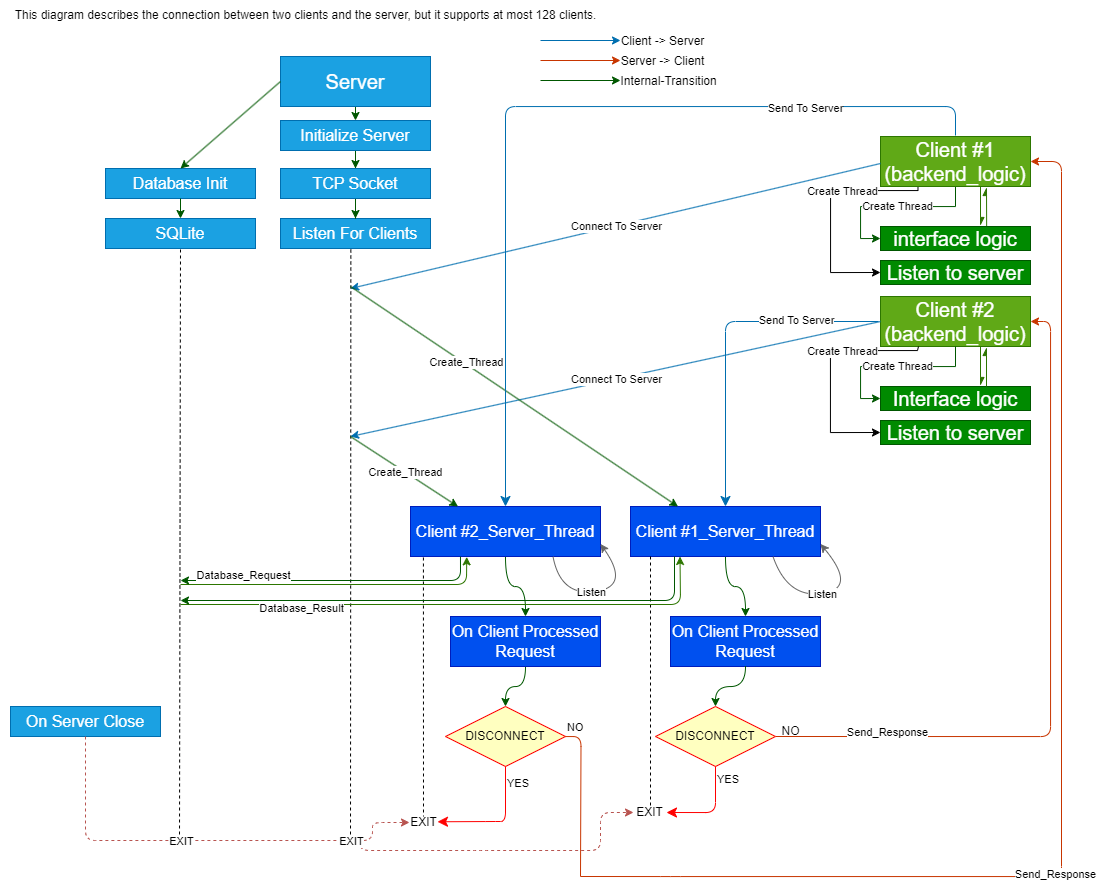
\includegraphics[scale=0.65]{tcp.png}
    \caption{Structura aplicației din punct al vedere al conecțiunii.}
    \label{fig:yourlabel}
\end{figure}



\newpage
{\Large Diagrama UML}

\begin{figure}[htbp!]
    \hspace{0px} 
    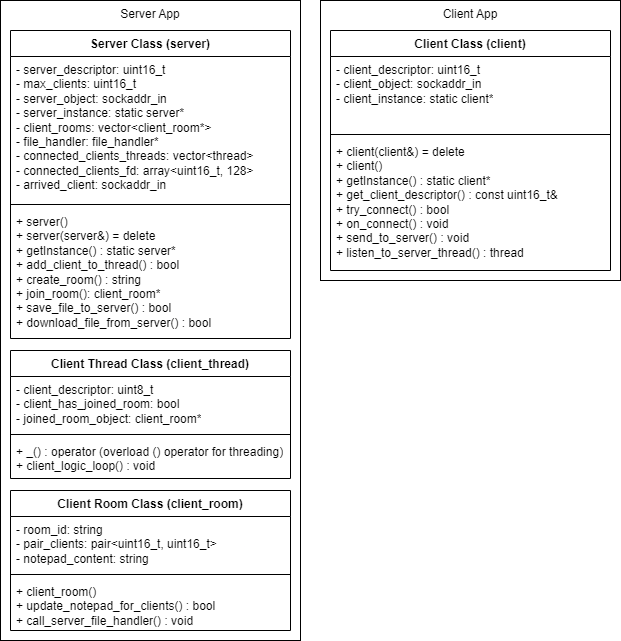
\includegraphics[scale=0.529]{uml.png}
    \caption{Clasele obiectelor folosite în aplicație.}
    \label{fig:yourlabel}
\end{figure}


\newpage
{\bf \large 3.1 Elemente cheie}
\\

{\bf \large Serverul}

Serverul este componenta care face legătura între toți utilizatorii. Acesta folosește drept protocol, protocolul {\bf TCP}, fiind necesară transmiterea
datelor într-un flux continuu, sigur. Serverul are drept design pattern {\bf singleton-ul}, asigurând existența unei singure instanțe per aplicație și totodată accesul global la aceasta.
Instanța se află pe thread-ul main, aceasta ascultând după noi posibile conecțiuni (accept(2)). În urma unei noi conecțiuni, serverul instanțiază, într-un thread nou, detașat,
un obiect de tipul (client\_thread), instanță specifică clientului conectat. 

Această instanță se ocupă în intregime de pri\-mi\-rea mesajelor de clientul respectiv, prelucrarea informațiilor și trimiterea unui răspuns. Folosirea multithreading-ului saturează nevoia concurenței serverului.

Instanțele respective sunt șterge din memorie la deconectarea clienților.
\\

{\bf \large Camera clienților}

Camera clienților este componenta care permite celor mult doi clienți să prelucreze fișiere simultan.
Un obiect de tipul (client\_room) se ocupă cu transmitirea datelor doar între utilizatorii conectați la cameră,
precum și conținul fișierului aflat în memoria serverului.

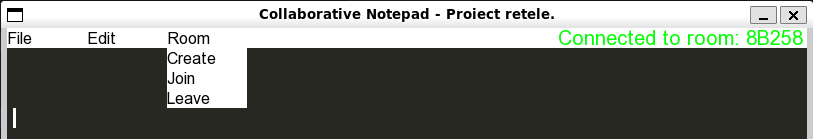
\includegraphics[scale=0.47]{camera.png}

Această componentă are mai multe funcționalități care pot fi accesate prin poziționarea cursorului pe butonul {\bf Room}.
\\

{\bf Creare cameră.} Un utilizator poate crea o cameră prin apăsarea butonului {\bf Create}. Utilizatorul va fi conectat imediat la camera creată,
cameră cu un ID alfa\-numeric de cinci caractere, generat aleatoriu. Interfața va specifica întotdeauna ID-ul camerei la care clientul este conectat.


{\bf Alăturare cameră.} Un utilizator poate să se alature unei camere prin apăsarea butonului {\bf Join}.

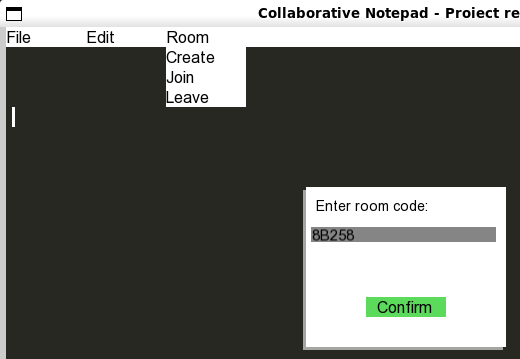
\includegraphics[scale=0.421]{camera2.png}

{\bf Părăsește camera.} Prin apăsarea butonului {\bf Leave} utilizatorul poate părăsi camera.

{\bf \large Managerul de fișiere}

Această componenta se ocupă cu manipularea fișierelor de către utilizatorii conectați la o cameră.

\begin{figure}[htbp!]
    \hspace{-8px} 
    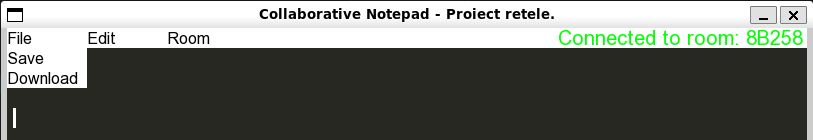
\includegraphics[scale=0.6]{camera3.png}
\end{figure}

Funcționalitățile pot fi accesate prin poziționarea cursorului pe butonul {\bf File}. De asemenea, utilizatorul poate manipula text-ul ca oricare alt notepad obișnuit prin apăsarea butonului
{\bf Edit}.
\\\\

{\bf Salvează fișier.} Un utilizator poate salva fișierul asociat camerei la care este conectat prin apăsarea butonului {\bf Save}. Fișierul este salvat în baza de date, utilizatorilor primind astfel
cod de identificare a fișierului, format din zece carac\-tere alfanumerice.
\\

{\bf Descarcă fișier.} Un utilizator poate descărca fișierul asociat camerei la care este conectat sau un fișier salvat în baza de date. Utilizatorul poate descărca fișierul la care lucrează în momentul respectiv, sau oricare alt
fișier prin introducerea unui cod de identificare format din zece caractere aflanumerice. Dacă în baza de date există un astfel de fișier, atunci utilizatorul îl poate descărca în orice loc din SO, oferindu-i-se această opțiune într-o căsuță pop-up.
\\

{\bf Deschide fișier.} Un utilizator poate deschide un fișier local prin apăsarea butonului {\bf Open}, fișier pe care ulterior îl poate asocia unei camere.
\\

{\bf Șterge fișier.} Un utilizator poate șterge un fișier aflat în baza de date prin identificarea acestuia cu ID-ul unic.
\\

\newpage
{\bf \large Clientul}
\\

Clientul reprezintă aplicația prin care utilizatorul poate interacționa cu serverul, acesta putând să facă schimb de date neintrerupt cu acesta.
Instanța clientului este formată din trei thread-uri cu funcționalități esențiale.

Thread-ul main este thread-ul care ascultă input-uri de la client, fie ele comenzi de la consolă sau cereri primite de la intefața grafică.
În momentul unei astfel de cereri, thread-ul trimite către server comanda, serverul o prelucrează, ulterior clientul citește răspunsul primit.

Al doilea thread constă într-un {\bf listener} care ascultă în permanență serverul, într-un mod neblocant, procesând orice mesaj primit de la server.

Al treilea thread reprezintă logica și funcționalitatea interfaței grafice.

Clientul trimite către server o dată la câteva secunde un {\bf heartbeat} pentru a se asigura că conecțiunea încă există.

\begin{figure}[htbp!]
    \hspace{-53px} 
    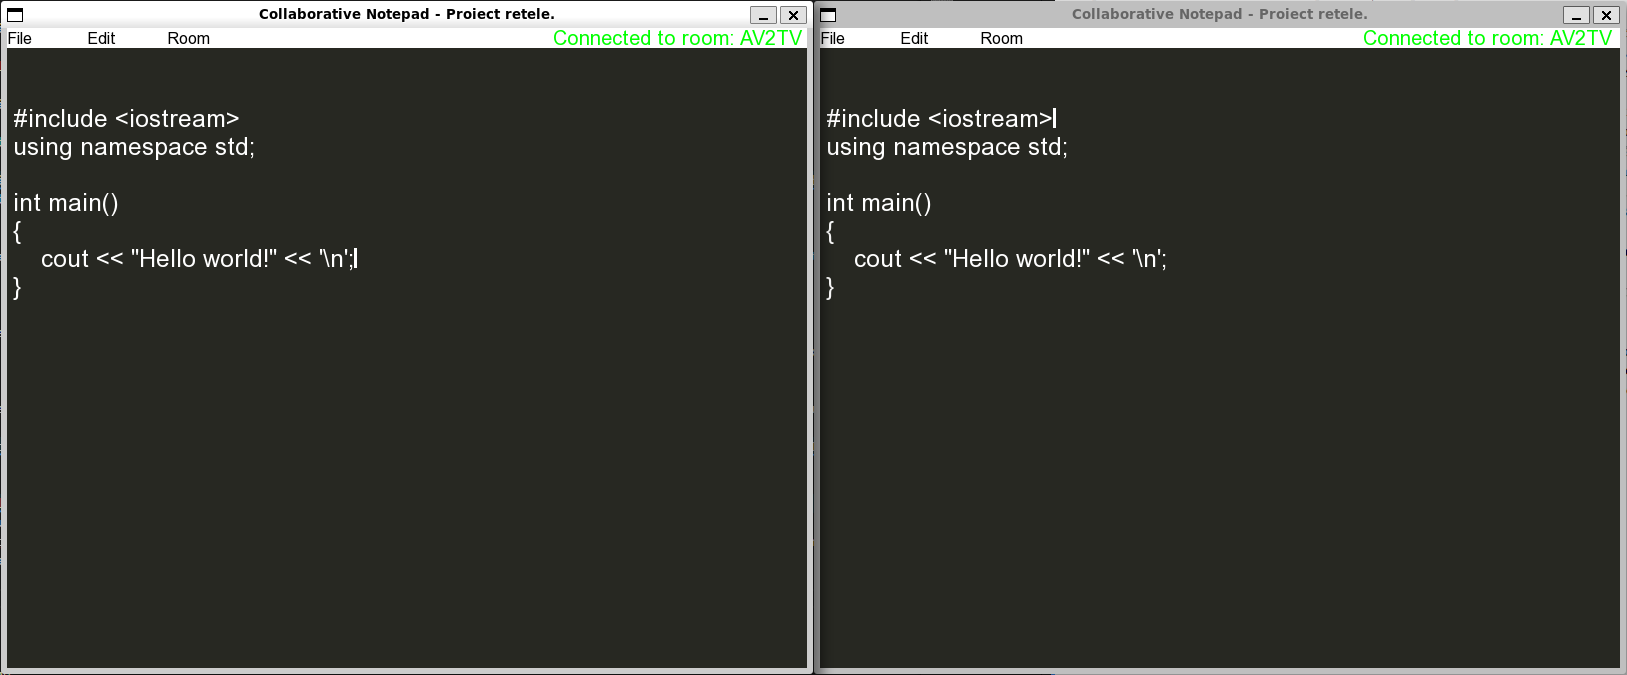
\includegraphics[scale=0.38]{camera4.png}
    \caption{Prototip al interfaței grafice scris în SFML.}
    \label{fig:yourlabel}
\end{figure}

\newpage
{\Large \bf 4 Aspecte de implementare} 
\\

Pentru acest proiect partea de server-client a fost implementată cu librăriile {\bf UNIX} (ex: sys/socket, netinet/ip.h) și drept {\bf design-pattern};
serverul și clientul sunt {\bf singleton}-uri pentru că orice instanță a aplicației client sau a aplicație server au, implicit, un singur client sau un singur server.

Mai jos este un snippet de cod care reprezintă inițializarea logicii thread-ului principal al serverului.
\\

{\large server.cpp}
\begin{tiny}
\begin{lstlisting}
    #define undefined -1

    ...

    int main()
    {
        signal_handler_logic();
        server* server_object = server::instance(AF_INET, SOCK_STREAM, 0, INADDR_ANY, 25565, 32);

        uint8_t connected_client_descriptor = undefined;

        std::vector<std::string> server_processing_thread_parameters;

        while(true)
        {
            socklen_t _l = sizeof(server_object->arrived_client);
            if((connected_client_descriptor = accept(server_object->get_server_descriptor(), reinterpret_cast<sockaddr*>(&server_object->arrived_client), &arrived_client_length)) == -1)
            {
                handle_error("Couldn't accept connection");
            }
            printf("Client with ID: %d has connected.\n", connected_client_descriptor);
            std::vector<std::string> thread_parameters;
            thread_parameters.push_back(std::to_string(connected_client_descriptor));
            std::thread connected_client_thread(client_thread(), thread_parameters);
            server_object->connected_clients_fds[++server_object->connected_clients_count] = connected_client_descriptor;
            connected_client_thread.detach();
        }
    printf("OK\n");
    }
\end{lstlisting}
\end{tiny}
\newpage

{\Large \bf 5 Concluzii}
\\

În concluzie, Collaborative-Notepad este un proiect complex, interesant cu uzabilitate în viața reală. Spre exemplu, doi indivizi pasionați
pot programa concomitent, acest lucru accelerând timpul de dezvoltare al unei aplicații. Un alt exemplu ar fi reprezentat de dorința a doi prieteni
de a compune o carte împreună, putând astfel să o creeze concomitent.

Este mult loc de îmbunătățiri și de adăugare a unor caracteristi noi și inovative aplicației. Spre exemplu, aplicația va putea permite, în viitor,
conectarea a mai multor clienți în aceeași cameră; sau distribuirea locației curente a cursorului fiecărui client.
\\



\renewcommand{\refname}{Referințe bibliografice} 
\begin{thebibliography}{8}
    
    \bibitem{ref_article1}
    Pagina cursului de rețele și calculatoare, UAIC - Facultatea de Informatică
    \url{https://profs.info.uaic.ro/~computernetworks/cursullaboratorul.php}
    
    \bibitem{ref_lncs1}
    Pagina profesorului îndrumător, profesorul de la seminar.
    \url{https://profs.info.uaic.ro/~georgiana.calancea/laboratories.html}

    \bibitem{ref_article1}
    Listă cu porturile TCP
    \url{https://en.wikipedia.org/wiki/List_of_TCP_and_UDP_port_numbers}

    \bibitem{ref_article3}
    Informații despre std::mutex
    \url{https://en.cppreference.com/w/cpp/thread/mutex}
    
    \bibitem{ref_article1}
    Informații legate de std::thread, precum și alte mici noțiuni.
    \url{https://cplusplus.com/reference/thread/thread/}

    \bibitem{ref_article3}
    Informații despre formatul LNCS \url{http://www.springer.com/lncs}.
    \end{thebibliography}

\end{document}